% Chapter 3

\chapter{چارچوب کاری پروژه}

این فصل به معرفی داده‌های مسئله و همچنین معرفی و بررسی کامل مدل پیشنهادی مبتنی بر معماری شبکه عصبی کانولوشن می‌پردازد. مضاف بر این، چارچوب\LTRfootnote{Framework} استفاده شده و محیط شبیه‌سازی نیز مورد بحث قرار می‌گیرد.

\section{مجموعه داده تعریف شده در مسئله}

این بخش، به بررسی داده‌های مورد استفاده در آموزش شبکه‌های عصبی و مدل پیشنهادی برای حل مسئله می‌پردازد. این داده‌ها و مدل پیشنهادی برای حل مسئله، بر اساس مجموعه‌داده CIFAR-10 و کتابخانه PyTorch تعریف شده‌اند.
مجموعه‌داده CIFAR-10 شامل 60,000 تصویر رنگی ۳۲ در ۳۲ پیکسل  در 10 کلاس مختلف با 6000 تصویر در هر کلاس است. این کلاس‌ها شامل هواپیما، اتومبیل، پرنده، گربه، گوزن، سگ، قورباغه، اسب، کشتی و کامیون هستند. از این تعداد تصاویر، 50,000 تصویر برای آموزش و 10,000 تصویر برای تست استفاده می‌شود. شکل \ref{cifar} نمایی از این کلاس‌ها را نشان داده است.

\begin{figure}[H]
    \centering
   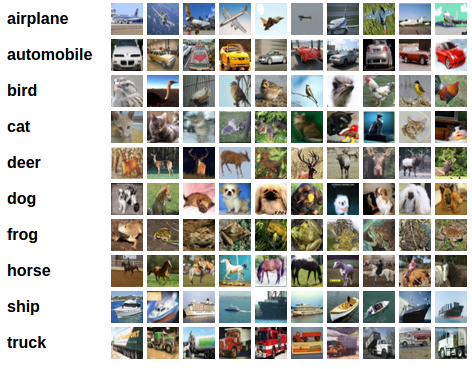
\includegraphics[height=10cm,width=12cm]{./cifar/cifar10.png}
   \caption{ نمونه‌ای از تصاویر دیتاست CIFAR10}
   \label{cifar}
   \centering
\end{figure}


برای آموزش شبکه عصبی، از کتابخانه PyTorch استفاده می شود. PyTorch یک کتابخانه یادگیری عمیق با قابلیت های بالا برای آموزش شبکه های عصبی است. در این پروژه، یک شبکه عصبی کانولوشنی تعریف شده و با استفاده از داده های آموزش CIFAR-10 آموزش دیده است. 
برای تعریف شبکه عصبی و آموزش آن، از تابع هزینه CrossEntropyLoss و الگوریتم بهینه سازی نزول گرادیان تصادفی\LTRfootnote{Stochastic Gradient Decent } با نرخ یادگیری \lr{0.001} استفاده شده است. تابع هزینه CrossEntropyLoss یک تابع هزینه مناسب برای مسائل طبقه بندی چند کلاسه است.


\section{مدل استفاده شده برای حل مسئله}

این مسئله از یک شبکه عصبی کانولوشن نسبتاً ساده بهره می‌گیرد. تابع فعال‌ساز\LTRfootnote{Activation Funcion} استفاده شده در هر لایه آن ReLU است که باعث پایداری شبکه می‌شود و رفتار خطی از خودش نشان می‌دهد.
شبکه دارای دو لایه کانولوشن و سه لایه تماماً متصل\LTRfootnote{Fully Connected Layar} است. در هر لایه کانولوشن، از یک لایه MaxPool2d برای کاهش ابعاد ویژگی‌ها استفاده می‌شود. سپس در هر مرحله ویژگی‌های سطح بالاتر استخراج می‌شوند تا نوبت به لایه‌های مخصوص به دسته‌بندی برسد. در نهایت بعد از استخراج ویژگی‌های منحصر به فرد هر تصویر و پیدا شدن مقدار احتمال حضور در هر یک از دسته‌ها، خروجی از طریق سه لایه تماماً متصل به یک بردار با ۱۰ عنصر تبدیل می‌شود که نشان‌دهنده احتمالات دسته‌بندی مختلف برای هر یک از کلاس‌های مجموعه داده است. نمودار مربوط به این شبکه در شکل \ref{CNN3} قابل مشاهده است.


\begin{figure}[h]
\usetikzlibrary{positioning, fit}
\resizebox{1\textwidth}{!}{%
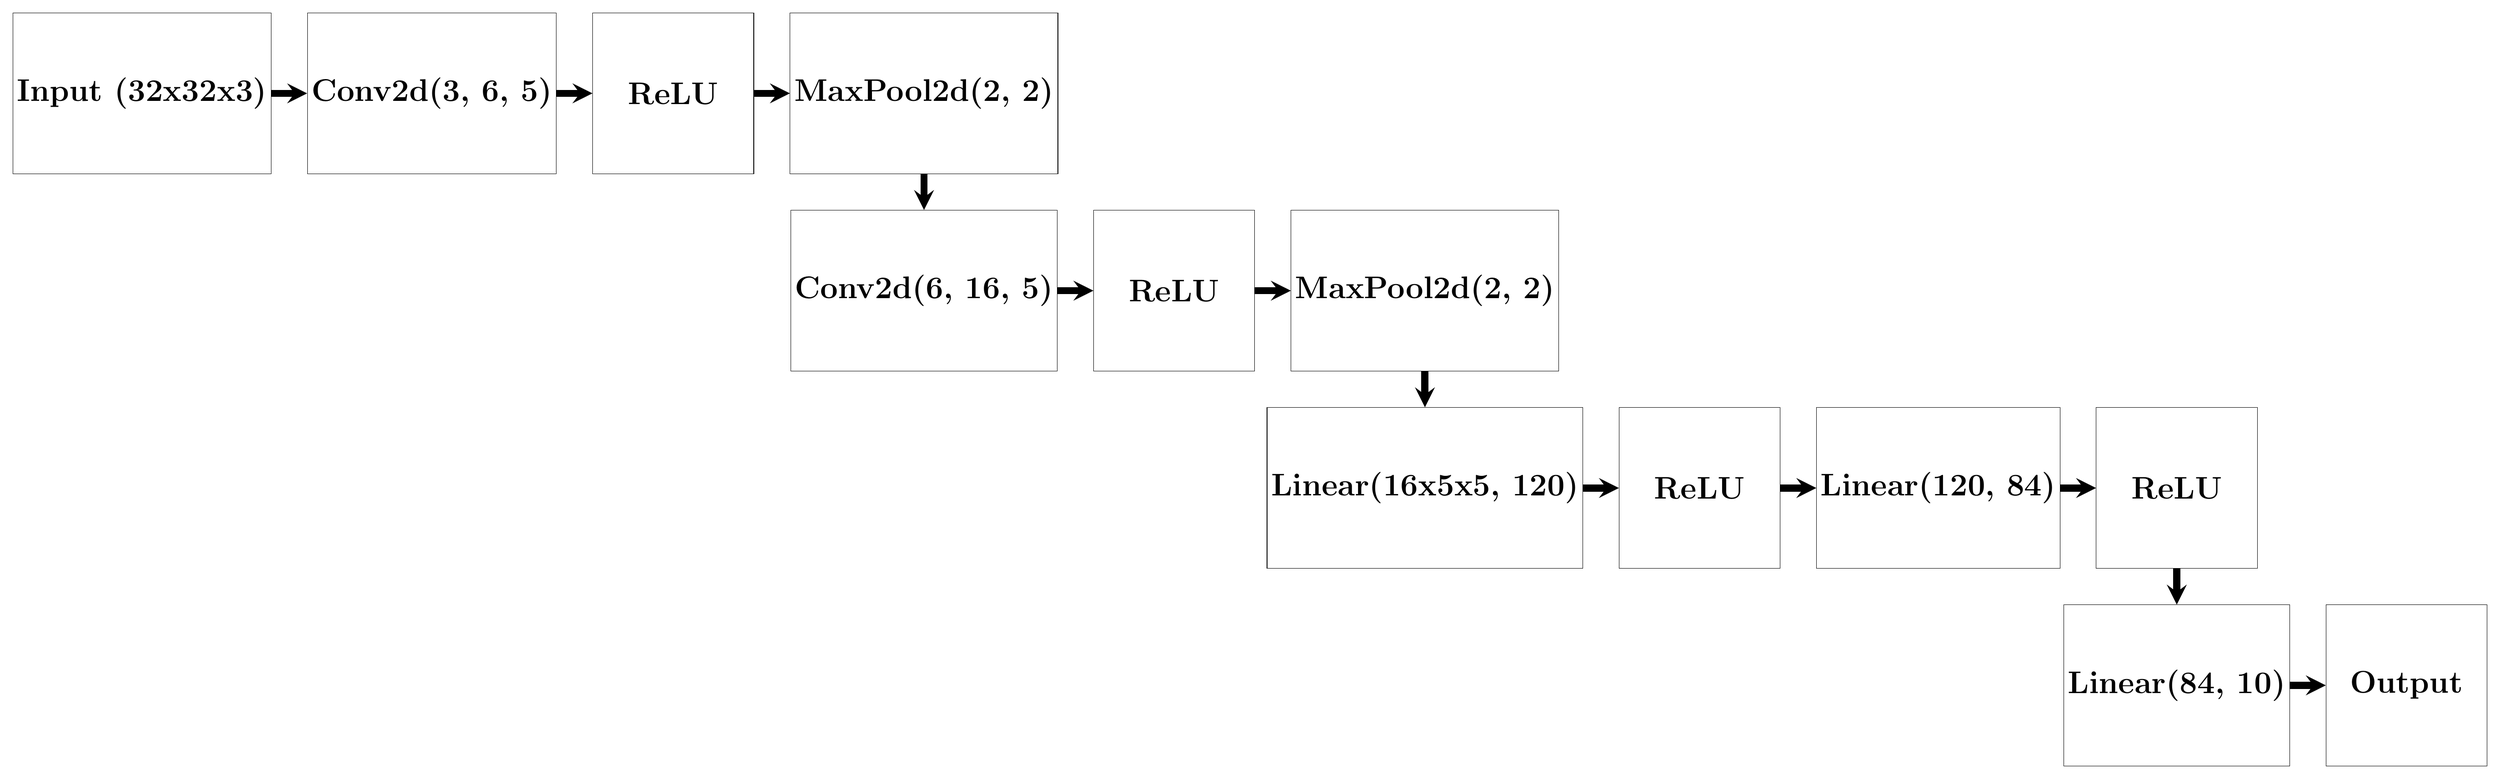
\begin{tikzpicture}[x=2.5cm, y=2.5cm, >=stealth, every node/.style={minimum size=4.5cm,font=\fontsize{50}{66}\selectfont\bfseries}]
   
        % nodes
\node [draw] (input) at (0,0) {\lr{Input (32x32x3)}};
\node [draw, right=of input] (conv1) {\lr{Conv2d(3, 6, 5)}};
\node [draw, right=of conv1] (relu1) {\lr{ReLU}};
\node [draw, right=of relu1] (pool1) {\lr{MaxPool2d(2, 2)}};
\node [draw, below=of pool1] (conv2) {\lr{Conv2d(6, 16, 5)}};
\node [draw, right=of conv2] (relu2) {\lr{ReLU}};
\node [draw, right=of relu2] (pool2) {\lr{MaxPool2d(2, 2)}};
\node [draw, below=of pool2] (fc1) {\lr{Linear(16x5x5, 120)}};
\node [draw, right=of fc1] (relu3) {\lr{ReLU}};
\node [draw, right=of relu3] (fc2) {\lr{Linear(120, 84)}};
\node [draw, right=of fc2] (relu4) {\lr{ReLU}};
\node [draw, below=of relu4] (fc3) {\lr{Linear(84, 10)}};
\node [draw, right=of fc3] (output) {\lr{Output}};

% arrows
\draw [->, line width=2mm] (input) -- (conv1);
\draw [->, line width=2mm] (conv1) -- (relu1);
\draw [->, line width=2mm] (relu1) -- (pool1);
\draw [->, line width=2mm] (pool1) -- (conv2);
\draw [->, line width=2mm] (conv2) -- (relu2);
\draw [->, line width=2mm] (relu2) -- (pool2);
\draw [->, line width=2mm] (pool2) -- (fc1);
\draw [->, line width=2mm] (fc1) -- (relu3);
\draw [->, line width=2mm] (relu3) -- (fc2);
\draw [->, line width=2mm] (fc2) -- (relu4);
\draw [->, line width=2mm] (relu4) -- (fc3);
\draw [->, line width=2mm] (fc3) -- (output);

\end{tikzpicture}
}
\caption{ساختار شبکه عصبی کانولوشن استفاده شده در مسئله ۱۰ کلاسه}
\label{CNN3}
\end{figure}
برای بهبود عملکرد شبکه، می‌توان از روش‌های مختلفی استفاده کرد. برای مثال، می‌توان تعداد فیلتر‌ها در لایه‌های کانولوشن را افزایش داد، یا از روش‌های منظم‌سازی مانند Dropout یا \lr{Batch Normalization} استفاده کرد. همچنین، می‌توان تابع فعال‌ساز ReLU را با توابع فعال‌ساز دیگری مانند LeakyReLU یا Sigmoid جایگزین کرد. در نهایت، میتوان شبکه را با داده‌های آموزش بسیار بیشتر و با استفاده از روش‌های بهینه‌سازی پیشرفته‌تر آموزش داد.

\section{محیط توسعه استفاده شده }

محیط‌های توسعه متعددی برای پیاده‌سازی سناریوهای مختلف تولید شده‌ است. به عنوان مثال در تراز صنعتی، چارچوب \lr{FATE} توسط محققین شرکت \lr{Facebook} توسعه پیدا کرده است\cite{a1}. نقطه قوت این محصول امنیت و ایمنی بالا و قابل اطمینان برای کاربردهای کلان صنعتی می‌باشد. محیط دیگری که برای کاربردهای عملی و سهولت در استفاده توسط مهندسین آلمانی توسعه یافته است، \lr{Flower} نام دارد\cite{b1}. 

\lr{FATE} و \lr{Flower} هر دو چارچوب‌های منبع‌باز\LTRfootnote{Open Source} هستند که به توسعه‌دهندگان اجازه می‌دهند سناریوهای گوناگون یادگیری فدرال را پیاده سازی کنند. \lr{FATE} روی فراهم آوردن چارچوب محاسبات امن برای پشتیبانی از اکوسیستم هوش مصنوعی فدرال تمرکز دارد، در حالی که \lr{Flower} در هدف فراهم آوردن رویکردی کاربرپسند به یادگیری فدرال که با هر چارچوب یادگیری ماشین و زبان برنامه نویسی سازگار است، قرار دارد. هر دوی این محیط‌ها ویژگی‌ها و قابلیت‌های منحصر به فرد خود را دارند، به طوری که توسعه دهندگان می توانند از بین این دو یکی را که بهترین گزینه برای نیاز‌های آن‌ها است، انتخاب کنند. در این پروژه به دلیل سهولت دسترسی و دسترسی در محیط‌های شبیه‌سازی مختلف و فراهم بودن مثال‌های متعدد از سناریو‌های پیش‌فرض از این محیط به عنوان ابزاری برای پیاده‌سازی یادگیری فدرال در اینترنت اشیاء استفاده شده است. قابل ذکر است که این محیط نیازهای مربوط به پیاده‌سازی شرایط متنوع را به خوبی برطرف می‌سازد. از ویژگی‌های بارز این محیط می‌توان به سازگاری کامل با کتابخانه‌ها و محیط‌های دیگر توسعه یادگیری ماشین و هوش مصنوعی از جمله \lr{Pytorch} و \lr{Tensorflow} اشاره نمود.

\begin{figure}[H]
    \centering
   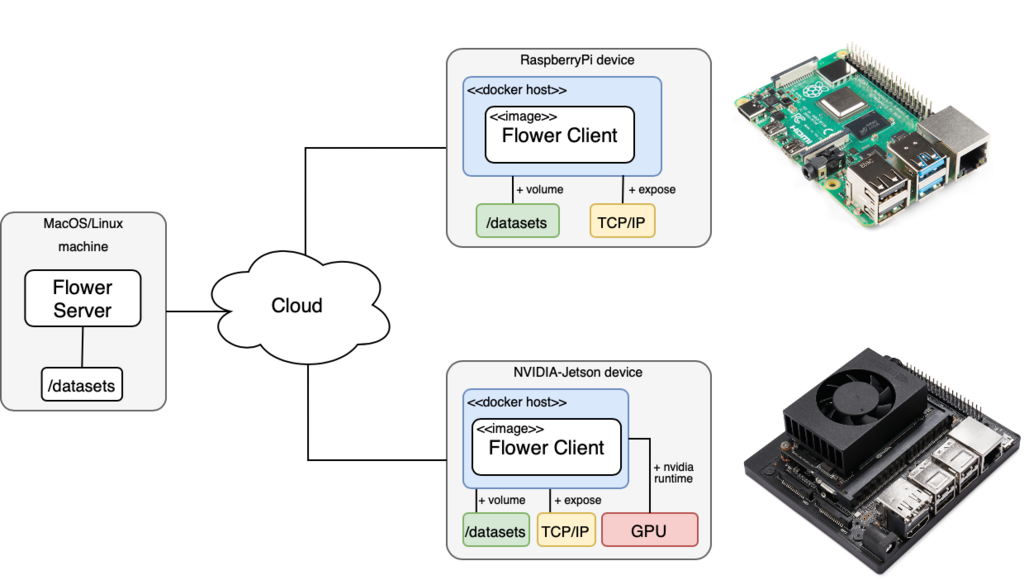
\includegraphics[height=8cm,width=10cm]{./Embedded/demo_diagram.png}
   \caption{ نمونه‌ای از پیاده سازی یادگیری فدرال روی دستگاه‌های تعبیه شده}
   \label{ pii }
   \centering
\end{figure}

برای پیاده‌سازی سرور لبه در دنیای واقعی نیز، مشابه سرور عمل می‌شود با این تفاوت که توان پردازشی می‌تواند تا حد امکان به اندازه‌ای که وقفه‌ای در مرحله یادگیری و آزمون صورت نگیرد، ساده‌تر در نظر گرفته شود.  الزاماً فرض بر این است که سرور لبه و سرور تجمیع‌کننده هر دو همیشه در شبکه فعال هستند و دائماً در حال گوش دادن روی یک پورت خاص به کارگران درخواست‌دهنده هستند. از طرف دیگر، کارگران که دستگاه‌های انتهایی هستند، می‌توانند با توجه به ماهیت کم‌توان بودن برای مصرف بهینه انرژی، به خواب‌های عمیق یا کوتاه‌مدت بروند. در عین حال سرور لبه می‌تواند به جای آن‌ها پاسخگوی سرور تجمیع‌کننده باشد تا گره دستگاه کم‌توان مجدداً به شبکه اضافه شود و پارامتر‌های خود را ارسال کند.

\section{پروتکل‌های انتقال داده در شبکه}

تقریباً تمامی چارچوبهای یادگیری فدرال از پروتکل امن\lr{gRPC}\LTRfootnote{gRPC Remote Procedure Calls} استفاده می‌کنند. \lr{gRPC} یک چارچوب متن‌باز و پر قدرت برای تماس‌های رویه‌ای از راه دور (RPC) است که توسط گوگل ایجاد شده است. این چارچوب قابلیت اجرا در هر محیطی را دارد و می‌تواند به طور کارآمد خدمات را درون و بین مراکز داده با پشتیبانی قابل‌تعویض برای توازن بار، ردیابی، بررسی سلامت و احراز هویت متصل کند. در این پروژه برای پردازش لبه از سرویس قدرتمند \lr{Nginx} استفاده شده است تا بتواند خواسته‌های مربوط به Proxy سرور را در لبه شبکه پوشش دهد.
از قابلیت‌های پیش‌فرض پلتفرم nginx پشتیبانی از این پروتکل است. همان‌طور که در شکل \ref{ grpc } نشان داده شده این پلتفرم می‌تواند به خوبی بسته‌\LTRfootnote{Packet}های grpc را انتقال بدهد. اما نکته حائز اهمیت آن است که ساختار بسته‌های grpc باید در هر دو طرف کلاینت و سرور کاملاً مشخص شده باشد (اصطلاحاً \lr{protobuf}). از آن‌جایی که nginx فاقد ساختار هر بسته است، تنها می‌تواند با استفاده از مشخصات داخل هدر فایل، اقدام به ارسال بسته کند. به عبارت دیگر، نمی‌توان به اطلاعات داخل بسته‌ها در وسط راه دسترسی پیدا کرد. البته از آن‌جایی که به صورت پیش‌فرض از این نوع بسته پشتیبانی می‌کند، قابلیت‌های خوبی در رابطه با مدیریت این نوع بسته قرار می‌دهد؛ مانند تعادل بار\LTRfootnote{Load Balancing} هنگام کار با چندین سرور به صورت همزمان و فشرده‌سازی\LTRfootnote{Compression} بسته‌های رد و بدل شده در شبکه.

\begin{figure}[H]
    \centering
   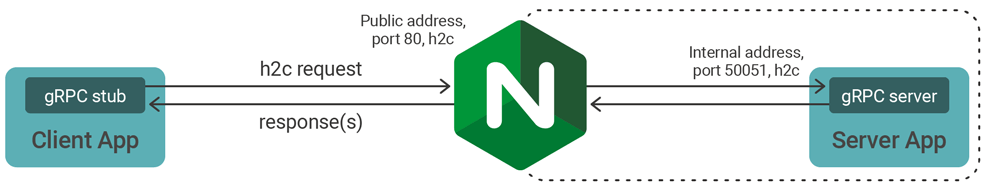
\includegraphics[height=4cm,width=14cm]{./GRPC/gRPC-nginx-proxy.png}
   \caption{ استفاده از nginx به عنوان پروکسی سرور}
   \label{ grpc }
   \centering
\end{figure}

میدانیم که nginx به خودی خود یک proxy server میباشد که در نگاه بالاتر با داشتن یک سرور لبه از نوع grpc میتوانیم به مراتب عملیات بیشتری در شبکه انجام بدهیم و با داشتن دیتای ارسالی کلاینت و سرور در لبه، در جدیدی از  قابلیت‌ها به روی مان باز خواهد شد.

\section{محیط شبیه‌سازی پیاده شده}

برای پیاده‌سازی سناریو ذکر شده از محیط قدرتمند شبیه‌سازی \lr{GNS3} استفاده شده است. در این محیط از دستگاه‌هایی با توان پردازشی محدود به‌عنوان کارگر و یک سرور مرکزی به‌عنوان تجمیع‌کننده استفاده شده است. همچنین از دستگاه‌هایی با توان پردازشی کمتر از سرور اصلی تجمیع‌کننده اما بیشتر از کارگران به‌عنوان مرکز پردازشی لبه استفاده شده است. شبکه داخلی حاوی سرور اصلی، کارگران و سرور لبه به‌عنوان یک شبکه اینترنت اشیاء مستقل که میتواند از پروتکل‌های مطرح شبکه‌های سنسوری بی‌سیم مثل بلوتوث مش\LTRfootnote{Bluetooth Mesh Sensor Networking} یا LORA\LTRfootnote{Long Range Wide Area} استفاده کند، پشت یک NAT\LTRfootnote{Network Address Translation} قرار دارد. تمامی این شبیه‌سازی‌ها بر روی یک لپ‌تاپ با ۱۶ گیگابایت رم و پردازنده ۸ هسته‌ای \lr{intel core i7} با فرکانس کاری ۳.۳ گیگاهرتز اجرا شده است. شکل \ref{scheme} بیانگر تصویری از این شبیه‌سازی می‌باشد.

\begin{figure}[H]
    \centering
   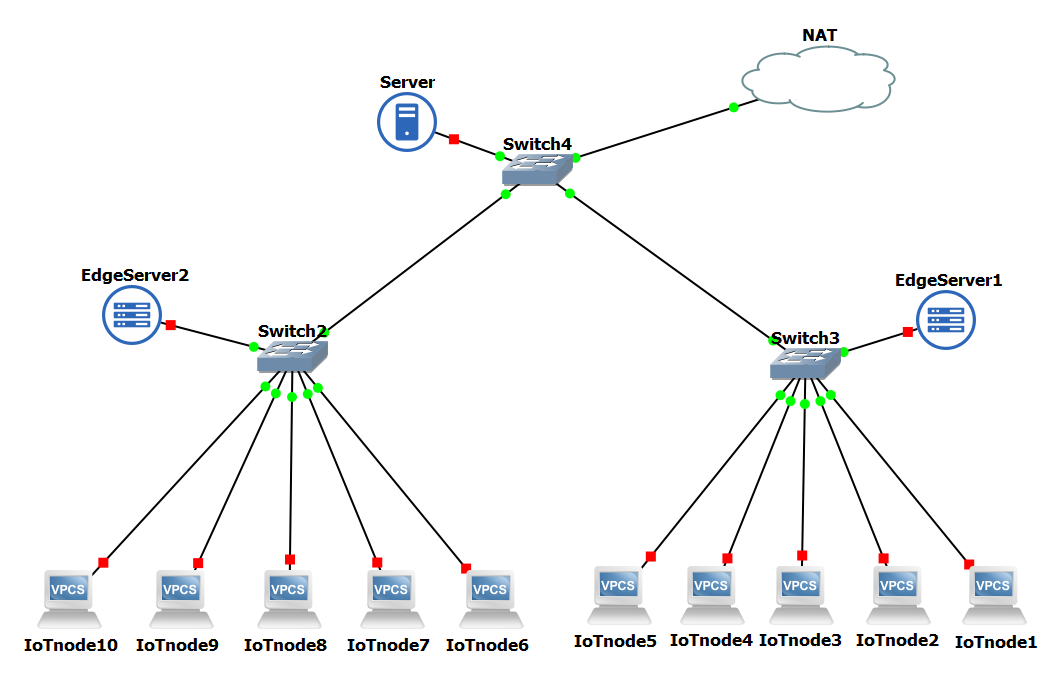
\includegraphics[height=8cm,width=14cm]{./GNS3/scheme.png}
   \caption{ محیط شبیه‌سازی شده در محیط نرم‌افزار \lr{GNS3}}
   \label{scheme}
   \centering
\end{figure}

\begin{figure}[H]
    \centering
   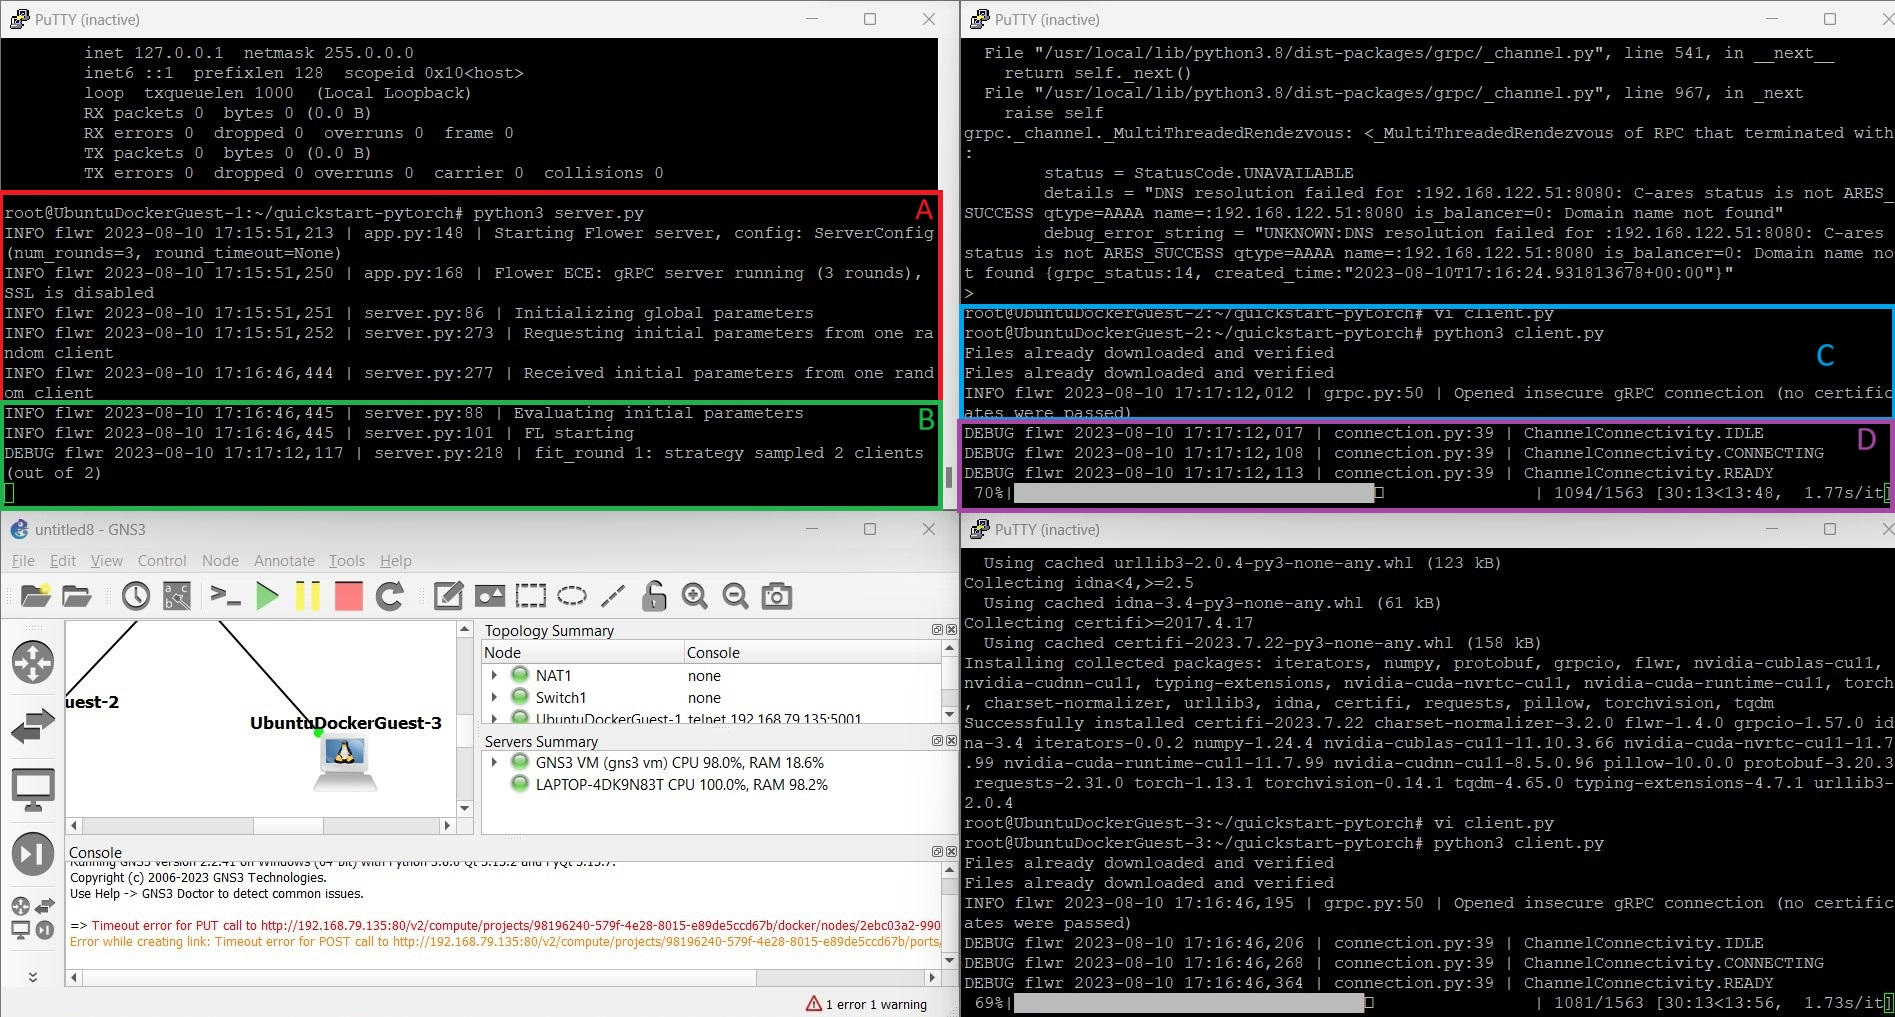
\includegraphics[height=12cm,width=16cm]{./GNS3/running.jpg}
   \caption{ نمونه‌ای از اجرای فرایند یادگیری و تست توسط یک شبکه ساده دارای دو کارگر}
   \label{running}
   \centering
\end{figure}


باتوجه به‌ شکل \ref{running}، قسمت‌های A و B مخصوص ترمینال سرور اصلی هستند و C و D نیز برای یکی از کارگران آورده شده‌اند. در ابتدا با اجرا شدن قسمت \lr{A}، سرور شروع به گوش دادن روی پورت و آدرس داده ‌شده (در اینجا آی‌پی آدرس سرور هاست در شبکه داخلی و روی یکی از پورت‌های آزاد معمولاً ۸۰۸۰) سپس منتظر می‌ماند تا تعدادی کارگر که حداقل آنها از قبل در کد برنامه تعریف شده به سرور وصل بشوند. سپس با رسیدن این تعداد به حداقل، فرآیند یادگیری آغاز می‌شود. وزن‌ها و بایاس‌های شبکه عصبی نیز در ابتدا در دور صفر از یکی از کارگران به صورت تصادفی دریافت می‌شوند (معمولاً اولین کارگری که وصل می‌شود). 
در کارگران نیز ابتدا با اجرا شدن کد برنامه در محیط سیستم عامل (در اینجا \lr{Ubunto})، ابتدا اقدام به دریافت فایل‌های مجموعه داده می‌کند که در اینجا از داده‌های CIFAR-10 استفاده شده است. پس از مبادرت به چک‌های اولیه از لحاظ معتبر بودن مجموعه داده و پیش‌نیاز‌های لازم، نوبت به ساخت کانال امن با استفاده از پروتکل GRPC می‌باشد. پس از رد و بدل کردن پیام‌های اولیه بر بستر \lr{HTTP2}، کانالی منحصر به فرد بین این کارگر و سرور اصلی ایجاد شده و تا پایان یادگیری باز می‌ماند. سپس بعد از وصل شدن کارگرهای بعدی به همین منوال، فرآیند در تمامی دستگا‌ه‌ها شروع می‌شود.

\begin{figure}[H]
    \centering
   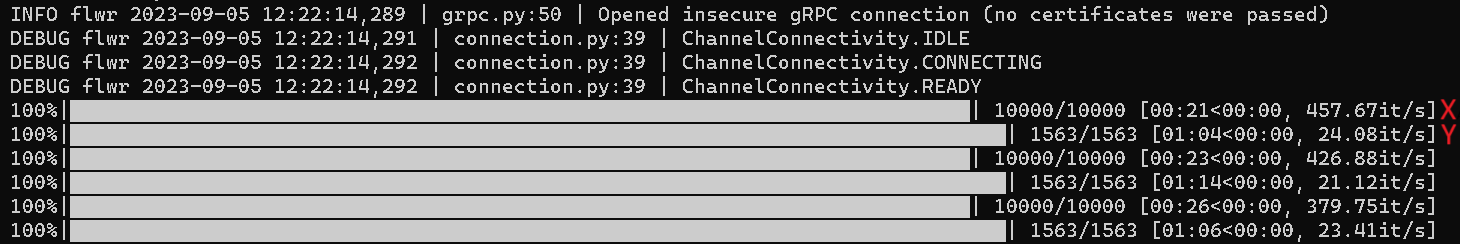
\includegraphics[height=4cm,width=16cm]{./simulations/client.png}
   \caption{ نمونه‌ای از کنسول یک کارگر در حال اجرای یادگیری فدرال}
   \label{client}
   \centering
\end{figure}


شکل \ref{client} نمونه‌ای از این فرآیند را در هر دور در هر کارگر با جزئیات بیشتری نشان می‌دهد. همان‌طور که مشخص است، مجموعه داده‌ CIFAR-10 شامل ۵۰ هزار تصویر آموزش و ۱۰ هزار تصویر تست است که باید توجه داشتیم که همان‌طور که از روی شکل شبیه‌سازی پیدا است، قسمت X بیانگر مرحله تست روی ۱۰ هزار عکس و مرحله Y بیانگر آموزش روی ۵۰ هزار تصویر این مجموعه داده می‌باشد. نکته قابل توجه این است که با توجه به اینکه اندازه هر batch برابر با ۳۲ است، با تقسیم ۵۰ هزار تصویر به ۱۵۳۲ دسته ۳۲تایی می‌رسیم تا در فرآیند آموزش از آن استفاده شود.

نکته دیگر مورد اهمیت این است که همان‌طور که توقع داریم، سرعت فرآیند آموزش به دلیل به‌روزرسانی شدن وزن‌ها در مدل از  فرآیند تست سریع تست و آخرین المان از هر خط  که به صورت تعداد عملیات بر ثانیه\LTRfootnote{Iteration Per Second} آمده است قرار دارد، با توجه به محدود بودن سخت‌افزاری در سیستم‌های اینترنت اشیاء، همان‌طور که از شکل \ref{running} واضح است، گاهاً این سرعت تا ۱ عملیات بر ثانیه کاهش پیدا می‌کند که این خود نشانی از اهمیت آن به عنوان گلوگاه اصلی در یادگیری فدرال در شبکه‌هایی با منابع محدود است.



%%%%%%%%%%%%%%%%%%%%%%%%%%%%%
